\chapter{\textbf{Queueing Network Model}}

The jobs identified in our Queueing Network Model are:
\begin{itemize}
\item StartUp Sampling Water Inland;
\item StartUp Sampling Water Outgoing;
\item Check Water Quality.
\end{itemize}

The first two jobs refer to the same Execution Graph.
In the diagram below you can see how the jobs interface with our system and how the nodes are interconnected with each other:

\bigskip
\begin{center}
\makebox[\textwidth]{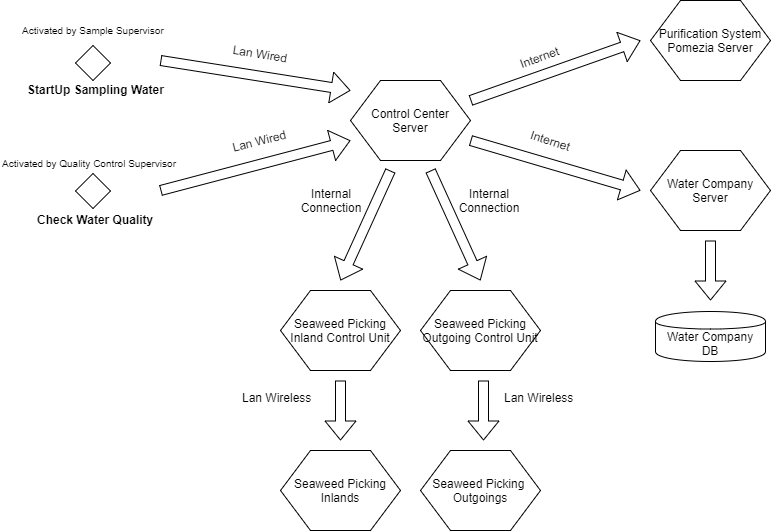
\includegraphics[width= 15cm]				{PhysicalNodes.png}}
\end{center}
\bigskip
\captionof{figure}{Physical Nodes}
\bigskip

This is the Queueing Network so obtained:

\begin{center}
\makebox[\textwidth]{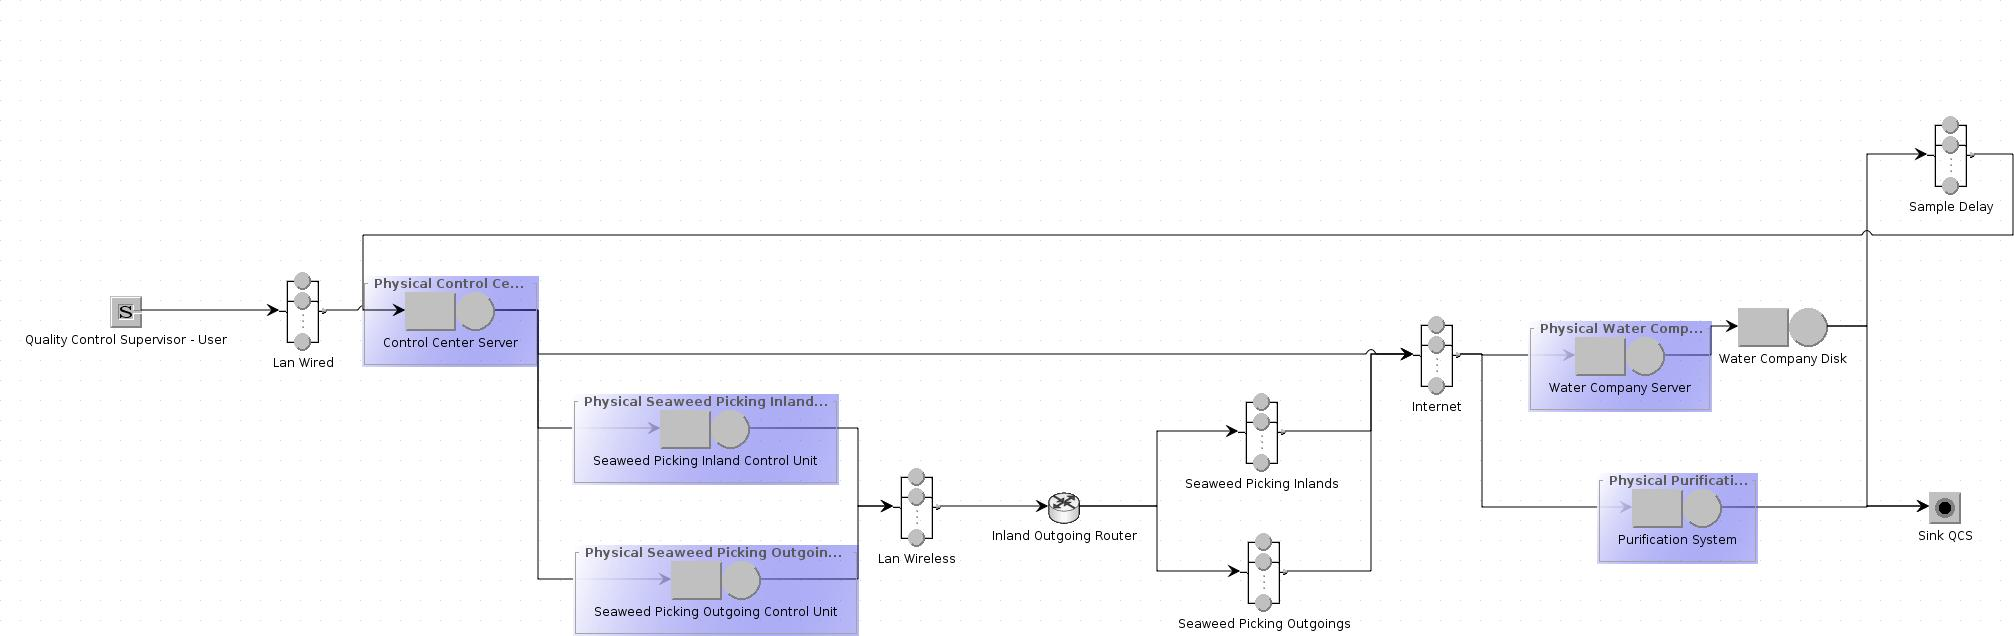
\includegraphics[width=\textwidth]				{QueueingNetwork.jpg}}
\end{center}
\bigskip
\captionof{figure}{Queueing Network}

Below physical nodes will be listed:
\begin{itemize}
\item Computational Nodes;
\begin{itemize}
	\item Control Center Server;
	\item SeaweedPicking Inland Control Unit;
	\item SeaweedPicking Outgoing Control Unit;
	\item Water Company Server;
	\item Purification System.
\end{itemize}
\item Node that store data:
\begin{itemize}
	\item Water Company Disk.
\end{itemize}	
\item Delay station that simulates Network delays:
\begin{itemize}
	\item Lan Wired;
	\item Lan Wireless;
	\item Internet.
\end{itemize}	
\item Delay station that simulates the sampling:
\begin{itemize}
	\item SeaweedPicking Inlands;
	\item SeaweedPicking Outgoing.
\end{itemize}
\item Delay station that simulates the deterministic interval time 		between sampling of the same Seaweed Picking:
\begin{itemize}
	\item Sample Delay.
\end{itemize}
\end{itemize}

\bigskip
After several tests, we agreed to reduce the sampling time to 500 ms to refine the performance analysis. On JMT for the same reason we have only one SeaweedPicking Control Unit with doubled performance and no two for In / Out.\\
We have also decided to eliminate the finite capacity regions as useless for the purposes of our project. \\
After other tests we have splitted each StartUp Sampling Water job into:
\begin{itemize}
	\item StartUp Sampling Water;
	\item Sampling.
\end{itemize}
This choice was driven by the fact that we did not know how many times the samples were made, as you can see in EG UC1.

\begin{center}
 \makebox[\textwidth]{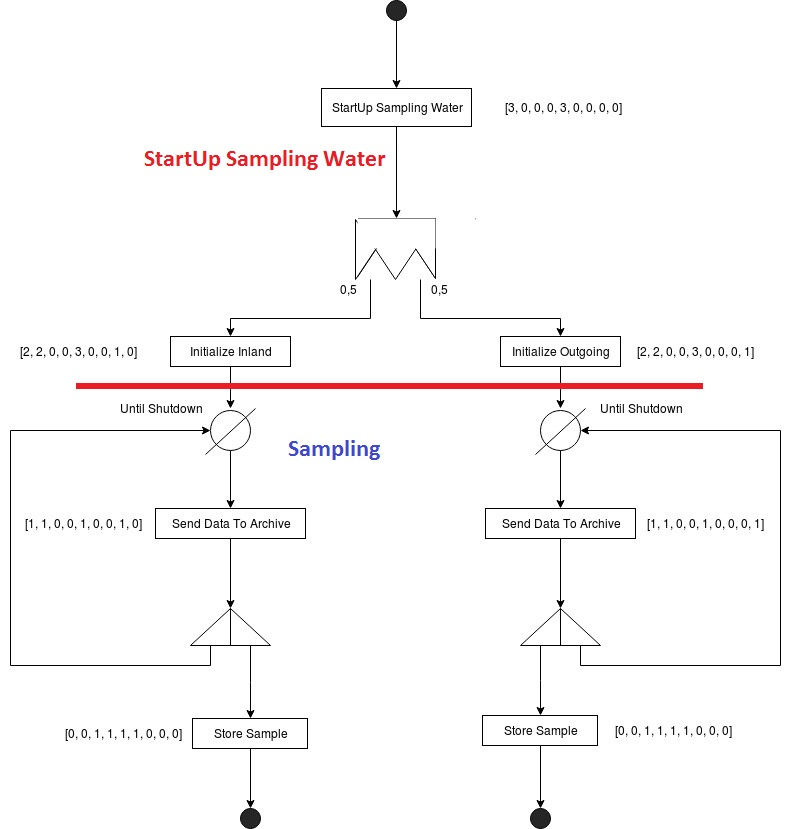
\includegraphics[width=14cm]				{SplittingStartUpSamplingWaterJob.jpg}}
\end{center}
\bigskip
\captionof{figure}{EG UC3 Check Water Quality}
\bigskip

For this purpose a Class Switch Node is introduced where each StartUp Sampling Water becomes a Sampling job.
So our final Queueing Network has become this:
 
\bigskip
\begin{center}
\makebox[\textwidth]{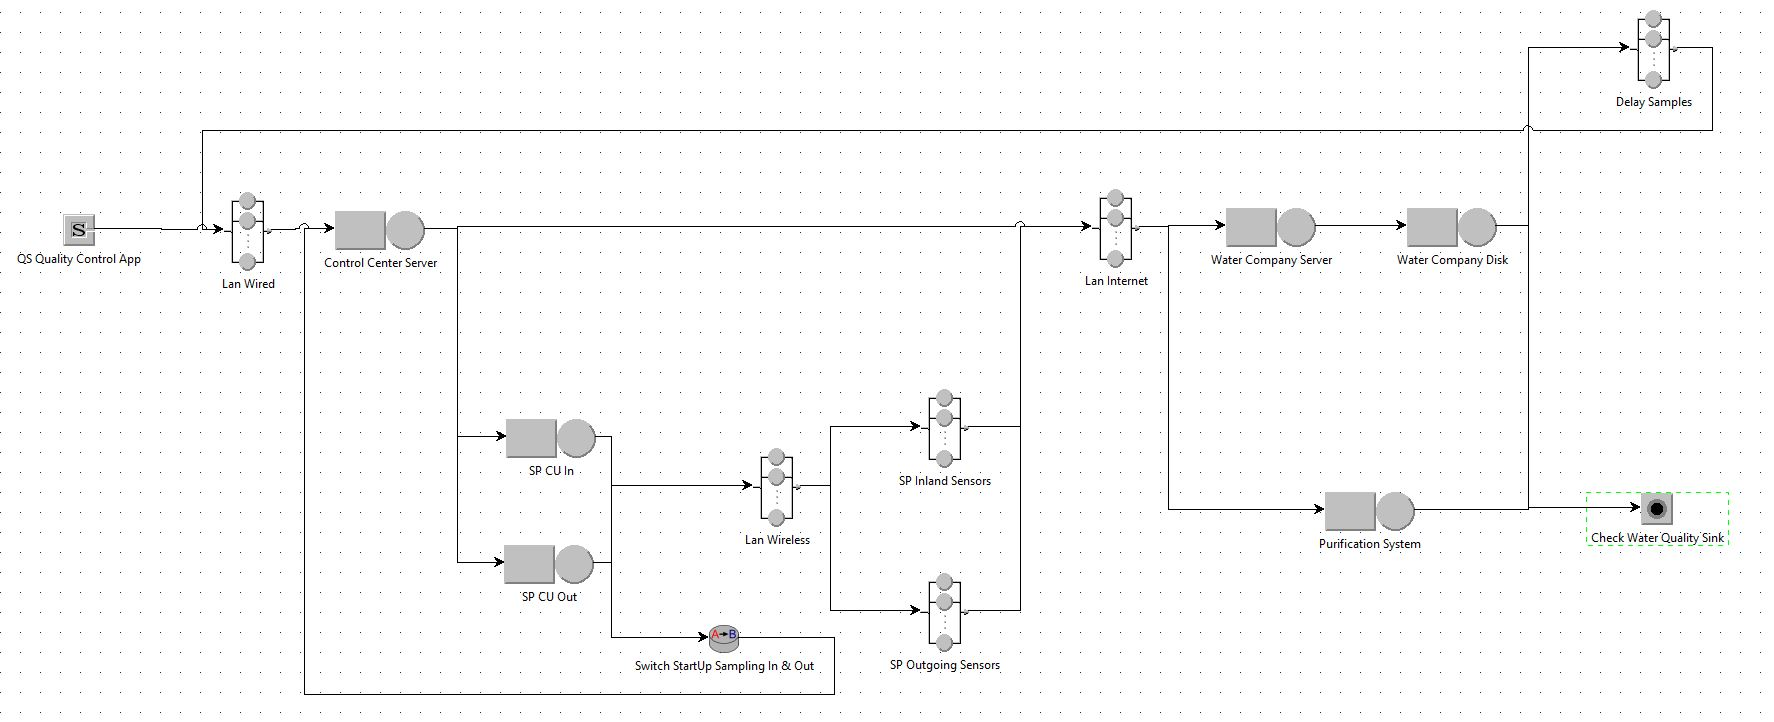
\includegraphics[width= \textwidth]				{QueuingNetworkFinal.jpg}}
\end{center}
\bigskip
\captionof{figure}{Final Queueing Network}



